\documentclass[10pt, a4paper]{article}
\usepackage[paper=a4paper, left=3cm, right=3cm, bottom=3cm, top=3.5cm]{geometry}
\usepackage{amsmath}
\usepackage{graphicx}
\usepackage{float}
\usepackage[latin1]{inputenc}
\usepackage[T1]{fontenc}
\usepackage[spanish]{babel}
\usepackage{footnote}
\usepackage{tikz}
\usetikzlibrary{"trees"}

\title{TP1 - Algoritmos y Estructuras de Datos III}
\date{2017-08-23}
\author{Catalina Gonzalo Juarros}

\begin{document}

\pagenumbering{gobble}

\maketitle

\newpage

\tableofcontents

\newpage

\pagenumbering{arabic}

\section{Problema a resolver}

	\subsection{Descripci\'on}

		Dado un conjunto de \textit{i} agentes, queremos determinar la \textbf{mayor cantidad de agentes confiables} en base a una secuencia de \textit{a} preguntas respondidas por ellos. Cuando un agente responde una pregunta, dice si otro agente -que puede ser \'el mismo- es confiable. Para cierto subconjunto de agentes, decimos que todos son confiables si y s\'olo si:
	
		\begin{itemize}
		\item Ning\'un agente del conjunto dice que alg\'un agente del conjunto no es confiable: si Ricardo dice que Rub\'en no es confiable pero tanto Ricardo como Rub\'en est\'an en el conjunto, este no es una soluci\'on v\'alida.
		\item Ning\'un agente del conjunto dice que un agente que est\'a fuera del conjunto es confiable: si Ricardo est\'a en el conjunto y dice que Rub\'en es confiable, obligatoriamente debemos agregar a Rub\'en.
		\end{itemize}
		
		Cada agente se caracteriza por un n\'umero $1 \leq n \leq i$ y cada pregunta respondida se representa con un par $(x,y): 1 \leq x,y \leq i$, donde \textit{x} es el agente que respondi\'o la pregunta, \textit{y} es el agente sobre el que \textit{x} respondi\'o y el signo de \textit{y} indica si \textit{x} dijo que \textit{y} es o no confiable (positivo es s\'i, negativo es no). Por ejemplo, el par $(1,2)$ se lee como ``1 dijo que 2 es confiable''. Siempre hay al menos un agente, pero puede no haber preguntas respondidas. Puede deducirse que en ese caso todos los agentes son confiables.
		
		Llamaremos a un conjunto de agentes del mayor tama\~no posible una \textit{soluci\'on \'optima}. En la secci\'on que sigue veremos ejemplos claros de soluciones \'optimas y casos en los que hay m\'as de una.
	
	\subsection{Ejemplos}
	
	\subsubsection{Caso 1}
	
		Analicemos las soluciones cuando tenemos 4 agentes y la secuencia de preguntas respondidas es $E = <(1,2), (1,-4), (2,-3), (3,1), (3,-4)>$:
		
		\begin{itemize}
		\item $<1, 2>$ es soluci\'on, ya que 1 dice que 2 es confiable. Observemos que $<1>$, entonces, no podr\'ia ser una soluci\'on. Observemos tambi\'en que no podemos extender nuestra soluci\'on, ya que 1 dice que 4 no es confiable y 2 dice que 3 no es confiable.
		\item $<2,4>$ tambi\'en es soluci\'on, porque a pesar de que 2 no dijo nada sobre 4, este subconjunto no rompe ninguna de las dos condiciones necesarias para ser una soluci\'on v\'alida. Tampoco podemos extenderla, por la misma raz\'on que la anterior.
		\item $<2>$ y $<4>$ son soluciones, pero obviamente no son \'optimas pues ya encontramos soluciones de 2 agentes.
		\end{itemize}
		
		Entonces, concluimos que la m\'axima cantidad de agentes confiables es 2. En este ejemplo se ve claramente que la soluci\'on \'optima \textbf{no necesariamente es \'unica}.
		
	\subsubsection{Caso 2}
	
		Veamos ahora qu\'e ocurre cuando tenemos un solo agente y la secuencia es $E = <(1,-1)>$:
		
		\begin{itemize}
		\item Observemos que una soluci\'on v\'alida \textbf{nunca} puede contener a 1, puesto que \'el mismo se considera no confiable.
		\item Pero 1 es el \'unico agente que tenemos, por lo que la \'unica soluci\'on v\'alida es el conjunto vac\'io.
		\end{itemize}
		
		En este caso hay una sola soluci\'on \'optima y la m\'axima cantidad de agentes es 0.


\section{Resoluci\'on}

%	\begin{figure}[H]
%		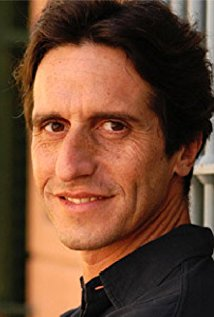
\includegraphics[width=100px]{peretti.jpg}
%		\caption{Diego Peretti.}
%		\label{peretti}
%	\end{figure}
%	
%	\begin{figure}[H]
%		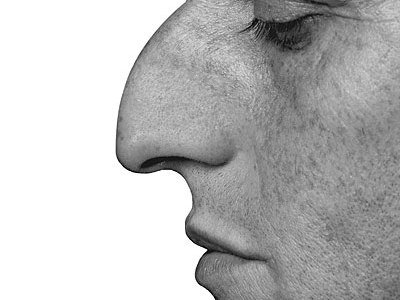
\includegraphics[width=150px]{nariz.jpg}
%		\caption{La nariz de Diego Peretti.}
%		\label{nariz}
%	\end{figure}
	
	\subsection{Idea}
	
	\subsubsection{Algoritmo}
		El algoritmo propuesto se basa en la t\'ecnica de \textit{backtracking}, que consiste b\'asicamente en:
		
		\begin{itemize}
		\item Construir una \textit{soluci\'on parcial} que pueda extenderse a \textbf{cualquier} soluci\'on candidata del problema en un n\'umero finito de pasos. Por ejemplo, si se intentara resolver un Sudoku, la soluci\'on parcial inicial podr\'ia ser ``dejar el tablero vac\'io'', y una extensi\'on consistir\'ia en llenar un casillero m\'as. En el problema presentado en este trabajo, la soluci\'on parcial inicial es el conjunto vac\'io, que se extender\'a a subconjuntos del conjunto total de agentes. \footnote{Observaci\'on: una soluci\'on parcial \textbf{no es} necesariamente una soluci\'on al problema. En el ejemplo del Sudoku, el tablero vac\'io no es una soluci\'on v\'alida, pero es posible llegar a una a partir de \'el mediante operaciones sencillas como llenar un casillero. Por el contrario, en el problema de los agentes, la soluci\'on parcial inicial \textbf{siempre} es v\'alida, aunque en muchos casos no ser\'a la \'optima.}
		\item Recorrer \textbf{todo} el espacio de soluciones v\'alidas o que podr\'ian extenderse a soluciones v\'alidas, a menudo mediante llamadas recursivas al mismo algoritmo. A partir de este esquema, puede modelarse el espacio de soluciones como un \textbf{\'arbol} donde cada nodo representa una soluci\'on parcial: la ra\'iz es la soluci\'on inicial y los hijos de cada nodo son las soluciones que pueden construirse directamente a partir de \'el. En este caso, el \'arbol es \textbf{binario}, la ra\'iz es el conjunto vac\'io y, para cada $(1 \leq j \leq i)$, el sub\'arbol izquierdo de un nodo de nivel $j-1$ representa los conjuntos que \textbf{no contienen al agente \textit{j}} y el derecho representa a los que \textbf{s\'i}. Por lo tanto, dado un nodo de nivel $j-1$ con una soluci\'on $S$, sus hijos representan decisiones a tomar: agregar a $j$ a $S$ y no agregar a $j$ a $S$.
		\item Elegir la soluci\'on \'optima entre las recorridas.
		\end{itemize}
		
		Es importante notar que un \'arbol de backtracking \textbf{no debe contener} soluciones candidatas que no puedan extenderse a soluciones v\'alidas. En el ejemplo del apartado 1, donde el conjunto de preguntas es $E = <(1,2), (1,-4), (2,-3), (3,1), (3,-4)>$, $<1>$ puede estar en el \'arbol, puesto que es posible extenderla a la soluci\'on v\'alida $<1, 2>$, pero $<1, 3>$ no, ya que no puede agregarse ning\'un agente que la haga v\'alida.
		
		El \'arbol de backtracking para este caso puede visualizarse as\'i:
		
		\tikzstyle{level 1}=[level distance=1cm, sibling distance=5cm]
		\tikzstyle{level 2}=[level distance=1cm, sibling distance=3.5cm]
		\tikzstyle{level 3}=[level distance=1cm, sibling distance=1.5cm]
		\tikzstyle{level 4}=[level distance=1cm, sibling distance=1.5cm]

		\tikzstyle{sol} = [text width=4em, text centered]
		\tikzstyle{end} = [text width=2em, text centered]
		
		\begin{center}
		
		\begin{tikzpicture}[grow=down, sloped]
		\node[sol] {$<>$}
		    child {
		        node[sol] {$<>$}        
		            child {
		                node[sol] {$<>$}
		                child {
		                  node[sol] {$<>$}
		                  child {
		                    node[sol] {$<>$}
		                  }
		                  child {
		                    node[sol] {$<4>$}
		                  }
		                  edge from parent
		                }
		                child {
		                  node[end] {\small inv\'alida}
		                  edge from parent
		                }
		                edge from parent
		            }
		            child {
		                node[sol] {$<2>$}
		                child{
		                  node[sol] {$<2>$}
		                  child{
		                    node[sol] {$<2>$}
		                    edge from parent
		                  }
		                  child{
		                    node[sol] {$<2,4>$}
		                    edge from parent
		                  }
		                  edge from parent
		                }
		                child{
		                  node[end] {\small inv\'alida}
		                  edge from parent
		                }
		                edge from parent
		            }
		            edge from parent 
		    }
		    child {
		        node[sol] {$<1>$}        
		        child {
		                node[end] {\small inv\'alida}
		                edge from parent
		            }
		            child {
		                node[sol] {$<1,2>$}
		                child {
		                   node[sol] {$<1,2>$}
		                     child {
		                       node[sol] {$<1,2>$}
		                       edge from parent
		                    }
		                    child {
		                      node[end] {\small inv\'alida}
		                      edge from parent
		                    }
		                   edge from parent
		                }
		                child {
		                  node[end] {\small inv\'alida}
		                  edge from parent
		                }
		                edge from parent
		            }
		        edge from parent         
		    };
		\end{tikzpicture}

		\end{center}

		Lo recorremos de izquierda a derecha: desde la ra\'iz, bajamos por la izquierda hasta llegar a la hoja $<>$, guardamos el valor 0 como la mayor cantidad de agentes encontrada y subimos al nivel 4. Como quedan m\'as hojas por revisar, miramos la hoja derecha $<4>$, y como su longitud es mayor a 0, actualizamos el m\'aximo valor encontrado. Ahora, como ya revisamos todas las hojas del nodo $<>$ en el nivel 4, subimos al 3 y vemos si hay un sub\'arbol derecho por explorar; no hay, y por lo tanto volvemos al 2. Repetimos esta l\'ogica hasta llegar a la ra\'iz y hacemos lo mismo con el sub\'arbol derecho. Entonces habremos chequeado todas las soluciones y tendremos la \'optima. Esta idea de \textbf{subir al nodo padre una vez que exploramos los sub\'arboles} es que lo que le da su nombre al \textit{backtracking} (en ingl\'es, ``seguir un mismo camino hacia atr\'as'').
		
		
		
		Adem\'as de estructurar el espacio de soluciones, el modelado de \'este como un \'arbol nos da una gran ventaja: es posible definir \textit{podas} que nos ayudan a recorrerlo m\'as inteligentemente y, en muchos casos, ahorrar llamadas recursivas y mejorar el rendimiento del algoritmo. Podemos imaginar una poda como ``cortar'' un determinado sub\'arbol del espacio de soluciones cuando sabemos que no contiene \textbf{ninguna soluci\'on mejor que la encontrada hasta el momento}, por m\'as que todos sus nodos sean soluciones parciales v\'alidas.
	
	\subsubsection{Poda 1}
	
	Supongamos que tenemos 4 agentes y el conjunto de encuestas es $E = <(1,2), (1,-3) >$. El \'arbol de backtracking tiene este aspecto:
	
	
	\begin{center}
		
		\begin{tikzpicture}[grow=down, sloped]
		\node[sol] {$<>$}
		child {
			node[sol] {$<>$}	
			child {
				node[sol] {$<>$}	
			}
			child {
				node[sol] {$<2>$}	
			}	
		}
		child {
			node[sol] {$<1>$}
		};
		\end{tikzpicture}

		\end{center}
	
	\subsubsection{Poda 2}
	
	\begin{center}
		
		\begin{tikzpicture}[grow=down, sloped]
		\node[sol] {$<>$}
		    child {
		        node[sol] {$<>$}        
		            child {
		                node[sol] {$<>$}
		                child {
		                  node[sol] {$<>$}
		                  child {
		                    node[sol] {$<>$}
		                  }
		                  child {
		                    node[sol] {$<4>$}
		                  }
		                  edge from parent
		                }
		                child {
		                  node[end] {\small inv\'alida}
		                  edge from parent
		                }
		                edge from parent
		            }
		            child {
		                node[sol] {$<2>$}
		                child{
		                  node[sol] {$<2>$}
		                  child{
		                    node[end] {\small podada}
		                    edge from parent
		                  }
		                  child{
		                    node[sol] {$<2,4>$}
		                    edge from parent
		                  }
		                  edge from parent
		                }
		                child{
		                  node[end] {\small inv\'alida}
		                  edge from parent
		                }
		                edge from parent
		            }
		            edge from parent 
		    }
		    child {
		        node[sol] {$<1>$}        
		        child {
		                node[end] {\small inv\'alida}
		                edge from parent
		            }
		            child {
		                node[sol] {$<1,2>$}
		                child {
		                   node[end] {\small podada}		                  
		                   edge from parent
		                }
		                child {
		                  node[end] {\small inv\'alida}
		                  edge from parent
		                }
		                edge from parent
		            }
		        edge from parent         
		    };
		\end{tikzpicture}

		\end{center}
	
	\subsection{Pseudoc\'odigo}

\section{Complejidad}

	\subsection{Caracterizaci\'on del peor caso}
	El algoritmo, como vimos en la secci\'on 2, consiste en probar subconjuntos de agentes hasta encontrar la m\'axima cantidad de informantes que pueden agregarse a la soluci\'on sin que uno contradiga a otro. Como es requisito que el arreglo que representa a cada subconjunto est\'e ordenado, s\'olo vamos a probar con \textbf{una} representaci\'on de cada subconjunto, por lo que la cantidad de soluciones posibles se corresponde con la cantidad de subconjuntos distintos de $\{1,...,i\}$ (es decir, el \textit{cardinal del conjunto de partes} de $\{1,...,i\}$). Este n\'umero es $2^{i}$. La justificaci\'on la voy a escribir cuando aprenda a hacer footnotes.
	\\
	En el peor caso, el algoritmo tiene que probar \textbf{todos} los subconjuntos, o sea $2^{i}$ soluciones candidatas. Lo voy a justificar cuando efectivamente haya hecho el algoritmo.

	\subsection{C\'alculo de complejidad}
	La complejidad de este algoritmo, en el peor caso, es

	\begin{equation*}	
	T(n) \in \mathcal{O}(2^{i} \times i^{2} \times \log{i} \times a )
	\end{equation*}
	
	\paragraph{Justificaci\'on}
	Dado que el algoritmo debe probar 

\section{C\'odigo fuente}

\section{Experimentaci\'on}

\end{document}